
\documentclass[annual]{acmsiggraph}

\usepackage{booktabs}
\usepackage{listings}

% code style for c

\RequirePackage[usenames,dvipsnames]{xcolor}

\definecolor{codeKeyword}{rgb}{0.00, 0.00, 1.00} 
\definecolor{codeComment}{rgb}{0.00, 0.50, 0.00} 
\definecolor{codeBkgnd}  {rgb}{0.95, 0.95, 0.95} 
\definecolor{codeFrame}  {rgb}{0.80, 0.80, 0.80} 

\definecolor{lightblue}  {rgb}{0.17, 0.57, 0.69}
\definecolor{darkgreen}  {rgb}{0.00, 0.50, 0.00}
\definecolor{lightgrey}  {rgb}{0.66, 0.66, 0.66}

\lstset
{
	language         = C
,	morekeywords     = {new, min, max, mix, floor, clamp, sign, uniform, texture2D, in, out, abs, pow, atan, acos, asin, sin, cos, dot, cross, length, textureSize2D, sampler2D, varying, return, const, for, if, true, false, sqrt }
,	sensitive        = true
,	basicstyle       = \footnotesize\ttfamily
,	backgroundcolor  = \color{codeBkgnd}
,	rulecolor        = \color{codeFrame}
,	keywordstyle     = \color{codeKeyword}
,	commentstyle     = \color{codeComment}
,	morecomment      = [l][\color{darkgreen}]{//}
,	morecomment      = [s][\color{darkgreen}]{/*}{*/}
,	morecomment      = [l][\color{lightblue}]{\#}
,	morecomment      = [s][\color{lightgrey}]{\"}{\"}
,	numberbychapter  = true
,	numbersep        = -4pt,
,	tabsize          =  4          
,	numbers          = none
,	numberstyle      = \tiny
,	frame            = single
,	framesep         =  4pt
, xleftmargin=\parindent
,	abovecaptionskip = \medskipamount
, firstnumber      = 1
, stepnumber       = 1,
,	emph             = { void, int, float, bool, vec2, vec3, vec4, ivec2, ivec3, ivec4, bvec2, bvec3, bvec4, mat2, mat3, mat4 }
,	emphstyle        = \color{lightblue} 
}

\usepackage{eso-pic}
\AddToShipoutPictureFG{\AtPageLowerLeft{\put(\LenToUnit{0.5\paperwidth},\LenToUnit{6mm}){\makebox[0pt][c]{\fontsize{6.5}{8}\selectfont\color{gray}Author's revised version (2026-11-14). Version of record: \url{https://doi.org/10.1145/2466533.2466550}}}}}

\TOGonlineid{45678}
\TOGvolume{0}
\TOGnumber{0}
\TOGarticleDOI{1111111.2222222}
\TOGprojectURL{}
\TOGvideoURL{}
\TOGdataURL{}
\TOGcodeURL{}

\newcommand{\scite}[1]{~\cite{#1}}

\title{Interactive Software Maps for Web-Based Source Code Analysis}

\author
{
	Daniel Limberger$^{~(a)}$
	\and
	Benjamin Wasty$^{~(b)}$
	\and
	Jonas Tr\"{u}mper$^{~(a)}$
	\and
	J\"urgen D\"ollner$^{~(a)}$
	\affiliation
	{
		\small{$^{(a)}$ Hasso-Plattner-Institut, University of Potsdam, Germany; e-mail: \{daniel.limberger, jonas.truemper, juergen.doellner\}@hpi.uni-potsdam.de}\\
 		\small{$^{(b)}$ Software Diagnostics GmbH, Potsdam, Germany; e-mail: benjamin.wasty@gmail.com}
 	}
}

\pdfauthor{Daniel Limberger, Benjamin Wasty, Jonas Tr\"{u}mper, J\"urgen D\"ollner}

\keywords{3D-Treemaps, Software Visualization, Computer Aided Analysis, Decision Making, Web Integration, WebGL}

\begin{document}

\teaser{
	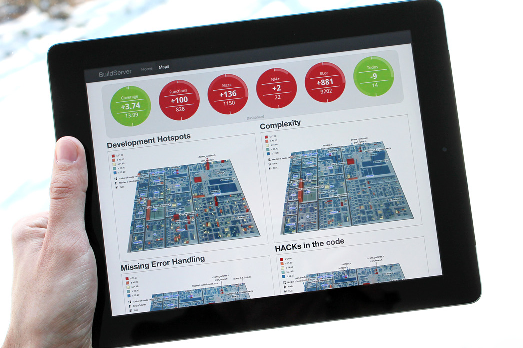
\includegraphics[width=.496\linewidth]{figures/dashboard2}
	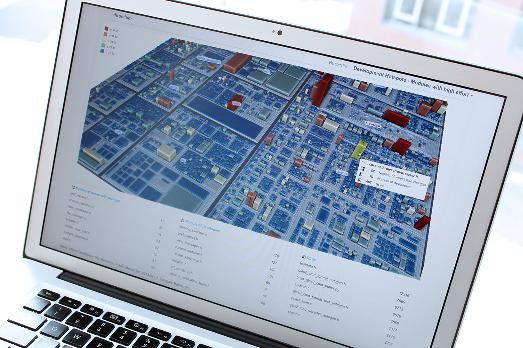
\includegraphics[width=.496\linewidth]{figures/prototype2clean}
	\caption{
	Left: Dashboard accessed from a tablet computer, which summarizes project-specific performance indicators (metrics) and links them to software maps.
	Right: Software map with code metrics mapped to ground area, height, and color, rendered in real-time in the browser. }
	\label{fig:teaser}
}

\maketitle

\begin{abstract}
\emph{Software maps} -- linking rectangular 3D-Treemaps, software system structure, and performance indicators -- are commonly used to support informed decision making in software-engineering processes.
A key aspect for this decision making is that software maps provide the structural context required for correct interpretation of these performance indicators.
In parallel, source code repositories and collaboration platforms are an integral part of today's software-engineering tool set, but cannot properly incorporate software maps since implementations are only available as stand-alone applications.
Hence, software maps are `disconnected' from the main body of this tool set, rendering their use and provisioning overly complicated, which is one of the main reasons against regular use.
We thus present a web-based rendering system for software maps that achieves both fast client-side page load time and interactive frame rates even with large software maps.
We significantly reduce page load time by efficiently encoding hierarchy and geometry data for the net transport.
Apart from that, appropriate interaction, layouting, and labeling techniques as well as common image enhancements aid evaluation of project-related quality aspects.
Metrics provisioning can further be implemented by predefined attribute mappings to simplify communication of project-specific quality aspects.
The system is integrated into dashboards to demonstrate how our web-based approach makes software maps more accessible to many different stakeholders in software-engineering projects.
\end{abstract}

\begin{CRcatlist}
  \CRcat{I.3.7}{Computer Graphics}{Three-Dimensional Graphics and Realism}{Virtual Reality}
	\CRcat{D.2.2}{Software Engineering}{Design Tools and Techniques}{Computer-aided software engineering};
  \CRcat{D.2.7}{Software Engineering}{Distribution, Maintenance, and Enhancement}{Documentation};
\end{CRcatlist}

\keywordlist

\vspace{-0.5pt}

\copyrightspace

\section{Introduction}

For a sustainable software engineering process in large software projects, a number of prerequisites exist.
These include good resource management, collaboration, code management, prioritization, reviews, and decision making as well as architecture- and feature planning.
Up-to-date knowledge of the software project, its processes, and, in particular, its source code is a further key element\scite{Eisenbarth2003}.
It is imperative to use additional services and platforms to support and ease this collaborative process\scite{Truemper2012}.
In fact, most available collaboration platforms provide visualization for various aspects related to development, e.g., branching, summary of development activities, status-related charts, source code diffs, and many more.

\begin{figure}[ht]
  \centering
  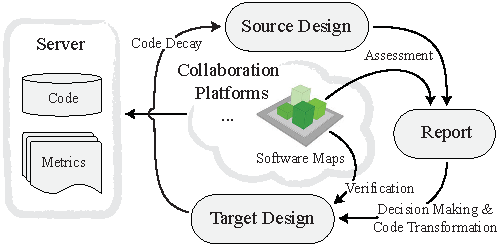
\includegraphics[width=1.0\linewidth]{figures/process}
  \caption{Exemplary development cycle within larger software engineering processes.
	Software maps as integrated part of collaboration platforms, which the development process relies on, aid assessment and verification.}
	\label{fig:process}
\end{figure}

With increasing project size, however, management overhead increases and an additional issue arises: Companies struggle with essential information gaps between management and development, which hinder informed decision making\scite{Poole2003}.
Such gaps include clearly communicating quality standards (management to development), and, vice versa, reasoning why a specific amount of resources is required for a given development task.
Visualizing these facts using traditional plain lists and charts is hard because of the exploratory nature of the underlying questions and problems:
It enforces an iterative refinement of and re-focusing within a massive amount of facts.
Fortunately, various powerful visualization techniques are available to help bridge this gap and to provide additional up-to-date information, which jointly aid exploring code quality, estimating benefits, and decision making.
Among others, code cities\scite{Wettel2007a} or software maps\scite{Bohnet2011} are frequently used in this context.
We here focus on software maps, which are 3D-Treemaps that provide a hierarchy-preserving layout and spatial context for code artifacts (\emph{code units}) and metrics.
Each treemap item represents a code unit (at varying abstraction levels) with at least three visual variables (height, ground area, color) that metrics can be mapped to.

While stand-alone applications for software maps, which allow arbitrary metric mappings, exist, their daily use in software engineering projects is significantly limited by several circumstances:
First and foremost, being stand-alone applications, they are \emph{disconnected} from the remainder of the preexistent tool set, so they impose an unnecessary usage overhead (e.g., context switches, data synchronization) on their users.
Second, provisioning such an application as per-computer stand-alone installation is complex, and, especially in industry contexts, requires the application to comply with company-specific security regulations etc.
Third, to enable any analysis benefits, specific knowledge not only about metrics is required, but also about how to express quality aspects as metric mappings \scite{Kitchenham1996}, which currently have to be configured per installation.
This can (partially) be alleviated by providing managers and developers with (initial) training that focuses on the company's individual engineering process(es), its requirements, and related quality issues \scite{Broy2006,Deissenboeck2009}.
Last, stand-alone applications cannot be integrated in web mashups, which further limits their use.

To overcome these drawbacks, we suggest integrating software-map related use cases into the (web-based) software engineering tool set, including tools such as collaboration platforms, frameworks, or web-interfaces of source code repositories (Figure \ref{fig:process}).
Hence, we \emph{connect} software maps to existing collaboration platforms by a web-based implementation that also centralizes metrics configuration.
Our system delivers fast loading times and interactive frame rates to ensure that the visualization does not interfere with the exploratory nature of the targeted use cases.
We achieve this by (1) introducing a method for efficient data provisioning, using JSON and Typed Arrays, for interactive visualization of software maps and 3D-Treemaps in general, including color encoding, normal generation, and geometry retrieval; (2) an image-based rendering pipeline implemented in JavaScript and WebGL that uses stylization techniques specialized on the visual exploration of code metrics through software maps, (3) an importance-based LOD-filtering for labeling, and (4) a set of interaction techniques specifically combined to support the given use case.
The system is accessible through WebGL-enabled \scite{Marrin2013} browsers, available on stationary and various types of mobile computers (e.g., tablets, notebooks, light desktop or office computers, etc. -- Figure \ref{fig:teaser}).
We demonstrate that our system scales up to real-world data, and evaluate its performance (provisioning, rendering) for integrated consumer graphics hardware.

\section{Related Work}

Visualization of data is in many aspects of high importance, providing meaningful insights for diverse groups of information consumers \scite{Langelier2005,Burger2007}.
As such, attributed 3D-Treemaps were suggested for software analysis, in the form of Code Cities \scite{Wettel2007a} or more recently as software maps \scite{Bohnet2011}.
The latter focus on aiding software engineering processes by monitoring certain source code aspects through metrics.
Similarly, integrating software maps with the common software-engineering tool set was suggested \scite{Truemper2012}, but focuses on using software maps as additional front-end for recommendation systems.

For the generation of treemap layouts, and thereby the provision of a spatial context to source code artifacts, various algorithms have emerged (e.g., \scite{Johnson1991}) for which an excellent resource for further exploration is available \scite{Schulz2011}.
For software maps we build on the strip treemap algorithm \scite{Bederson2002} that among others, was recently evaluated and improved \scite{Tak2012}.
While designing our web-based visualization and its data encoding, we evaluated state-of-the-art technologies \scite{Behr2010,Behr2012}, but neither fitted our needs for exclusively rendering software maps;
e.g., the additional latency introduced by requiring multiple requests to access distributed precision data over multiple textures seems inappropriate, and requires further investigation for various use cases.
Similarly, progressive (or LOD based) data provisioning \scite{Alliez2001} is impractical, unless it is desired to provide geometry data per hierarchy level and thereby allowing stepwise software map refinement.

Concerning efficient rendering of software maps or 3D-Treemaps in general, a technique utilizing geometry shaders was recently proposed \scite{Trapp2013}.
In WebGL, however, geometry shaders are not yet available, so we use basic rendering via attribute arrays. 
The suggested techniques as unsharp masking \scite{Luft2006}, edge-enhancement \scite{Nienhaus2003}, or use of camera lights, are directly integrated into our deferred rendering.
In addition, screen space ambient occlusion techniques, e.g., \scite{McGuire2010}, increase the perceived plasticity of software maps, aiding perception through better item and module differentiation and depth cues. 
Due to the limitations of WebGL, several tricks for data encoding into attribute arrays or G-Buffers (e.g., for texture encoding ids and depths), similar to \scite{Jung2013}, are necessary.

The problem space of labeling 3D-Treemaps is similar to the labeling of geovirtual 3D environments, hence, several works can be found.
We especially relate to the labeling approach introduced by \scite{Hagedorn2007}.
Labeling of empty spaces (i.e., due to padding) between modules as in \scite{Maass2007} is not used, since a meaningful orientation and unambiguous placement of labels seems not possible.
Though not implemented, the layouting by \scite{Lu2008} seems promising for better label placement in software maps.
Recently suggested approaches to overcome occlusion of labels in 3D navigation maps \scite{Vaaraniemi2012} might similarly enhance perceptibility of labels in 3D-Treemaps.

\section{Concept and Design}

\begin{figure}[t]
  \centering
  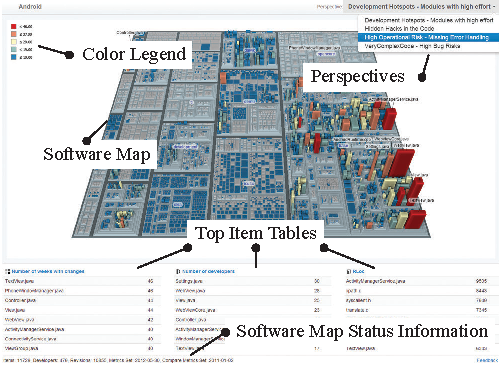
\includegraphics[width=1.0\linewidth]{figures/webinterfaceclean}
  \caption{The user interface of our web front-end, composed using HTML5 and CSS, comprises the following UI elements:
	The software map visualization itself as centerpiece offers a large area for exploration, a color legend for providing a context to the software-map's color mapping,
	and in the upper right the selection of predefined perspectives.
	For each of the three metrics some of the most important code units are listed below the visualization, enabling batch-highlighting individual code units in the software map.}
	\label{fig:webinterface}
\end{figure}

For our system, two instruments build orthogonal entry points for any subsequent exploratory analysis: (1) \emph{perspectives} and (2) \emph{dashboards}, which are outlined next.

\begin{enumerate}

	\item A perspective is a named, predefined set of metric mappings for software maps, by which for each of the three available visual attributes of the treemap items (resp. \emph{code units}) -- color, height, and ground area -- a metric can be selected.
	Such perspectives are defined in the context of a software project and allow for analyzing different aspects of the code base.
	Additionally, time or revision parameters, labeling configuration, and further parameters are specified.
	Other perspectives can be selected at run-time, triggering a reconfiguration of the software map.

	Since each perspective focuses on a specific set of metrics (or code aspect), expert users (i.e., lead developers and architects) typically reconfigure the software map multiple times (by selecting other perspectives) during an exploration session to correlate those aspects.
	Expert analysis with software maps is a highly iterative and exploratory process that is executed for building up and verifying hypotheses by examining orthogonal aspects of the code base\scite{Truemper2012}.
	Hence, fast perspective switching is an essential non-functional requirement for any system implementing software maps to ensure good user experience.

	\item A dashboard provides an overview of best or worst performers for a number of preselected metrics.
	Our implementation displays (1) lists of important code units, whose importance is given by predefined metrics (or perspectives) that are relevant to the individual software engineering process, and (2) up-to-date snapshots of all available perspectives using a default camera position. The snapshots enable direct jumps to related perspectives for further exploration. Further, (3) circular status indicators (inspired by a bootstrap template\scite{Perfectum2013}) give additional visual cues for specific metrics and further improve fast inspection and software map selection.

	In contrast to perspectives, dashboards typically function as entry point for managers to gain quick overview of key performance indicators (KPIs), and occasionally lead to in-depth analysis of those aspects by means of individual perspectives.

\end{enumerate}

In this paper, we only briefly outline the usage of entry point 2, dashboards, and focus on the use of entry point 1, perspectives.
Hence, users begin their interactive exploration session by selecting a perspective.
Subsequently, the software map is updated by handling layout changes, rendering the 3D-Treemap, coloring and labeling relevant code units.

A perspective is generally defined by selecting three metrics from a multitude of code metrics.
Here, metrics can be either common code metrics (e.g., lines of code) or project-specific metrics (e.g., aggregated metrics or style guide specifics).
When a metric is assigned to one of the treemap attributes, specific mapping parameters are configured.
For color mapping either a discrete or continuous color scheme is required.
Height mapping is accomplished through a scale function with a predefined maximum height.
Area mapping is also specified by an arbitrary scale function, controlling the code units' relative base area.
In addition to defining the mapping, various kinds of filters can be applied, e.g., for viewing all items touched by a certain author or team or all revisions referencing a certain bug.
All in all, defining perspectives is an expert task that requires a good understanding of available metrics and the respective aspect of the code base that is to be modeled by such perspective.

Once a perspective is defined and applied, we continue by rendering the software map and handling user interaction with it.
For our first prototypes we evaluated several WebGL Engines: ThreeJS, SceneJS and PhiloGL.
ThreeJS and SceneJS would have needed much customization, and matching our performance needs in their rendering pipeline would have caused similar effort as our custom implementation.
Due to SceneJS's scene graph and draw list implementation, no interactive frame rates were achieved for rather small software maps.
Finally, PhiloGL, as an easily extensible, fast, and lightweight engine, seems to fit best for this task.

The presented system, however, utilizes no third parties for rendering nor for generalized scene graph management. 
The WebGL canvas is integrated into HTML and also supports alpha blending, therefore allowing to place other, arbitrary HTML elements before or behind the visualization.
This is used to display a color legend and text labels for code units without the need to render them within the software map's virtual 3D space.

In the following sections we focus on server-side data provisioning, through efficient geometry and hierarchy data encoding, for browser based rendering.
For this, OpenCTM \scite{OpenCTM2013} was evaluated as a carrier format, but, especially for our data, a more efficient data encoding is obtainable.
The visualization process is presented in more detail, G-Buffer encoding schemes are provided, and adjustments made to treemap layouting and labeling, as well as interaction specifics are described.

\section{Software-Map Data Provisioning}

\begin{figure}[t]
  \centering
  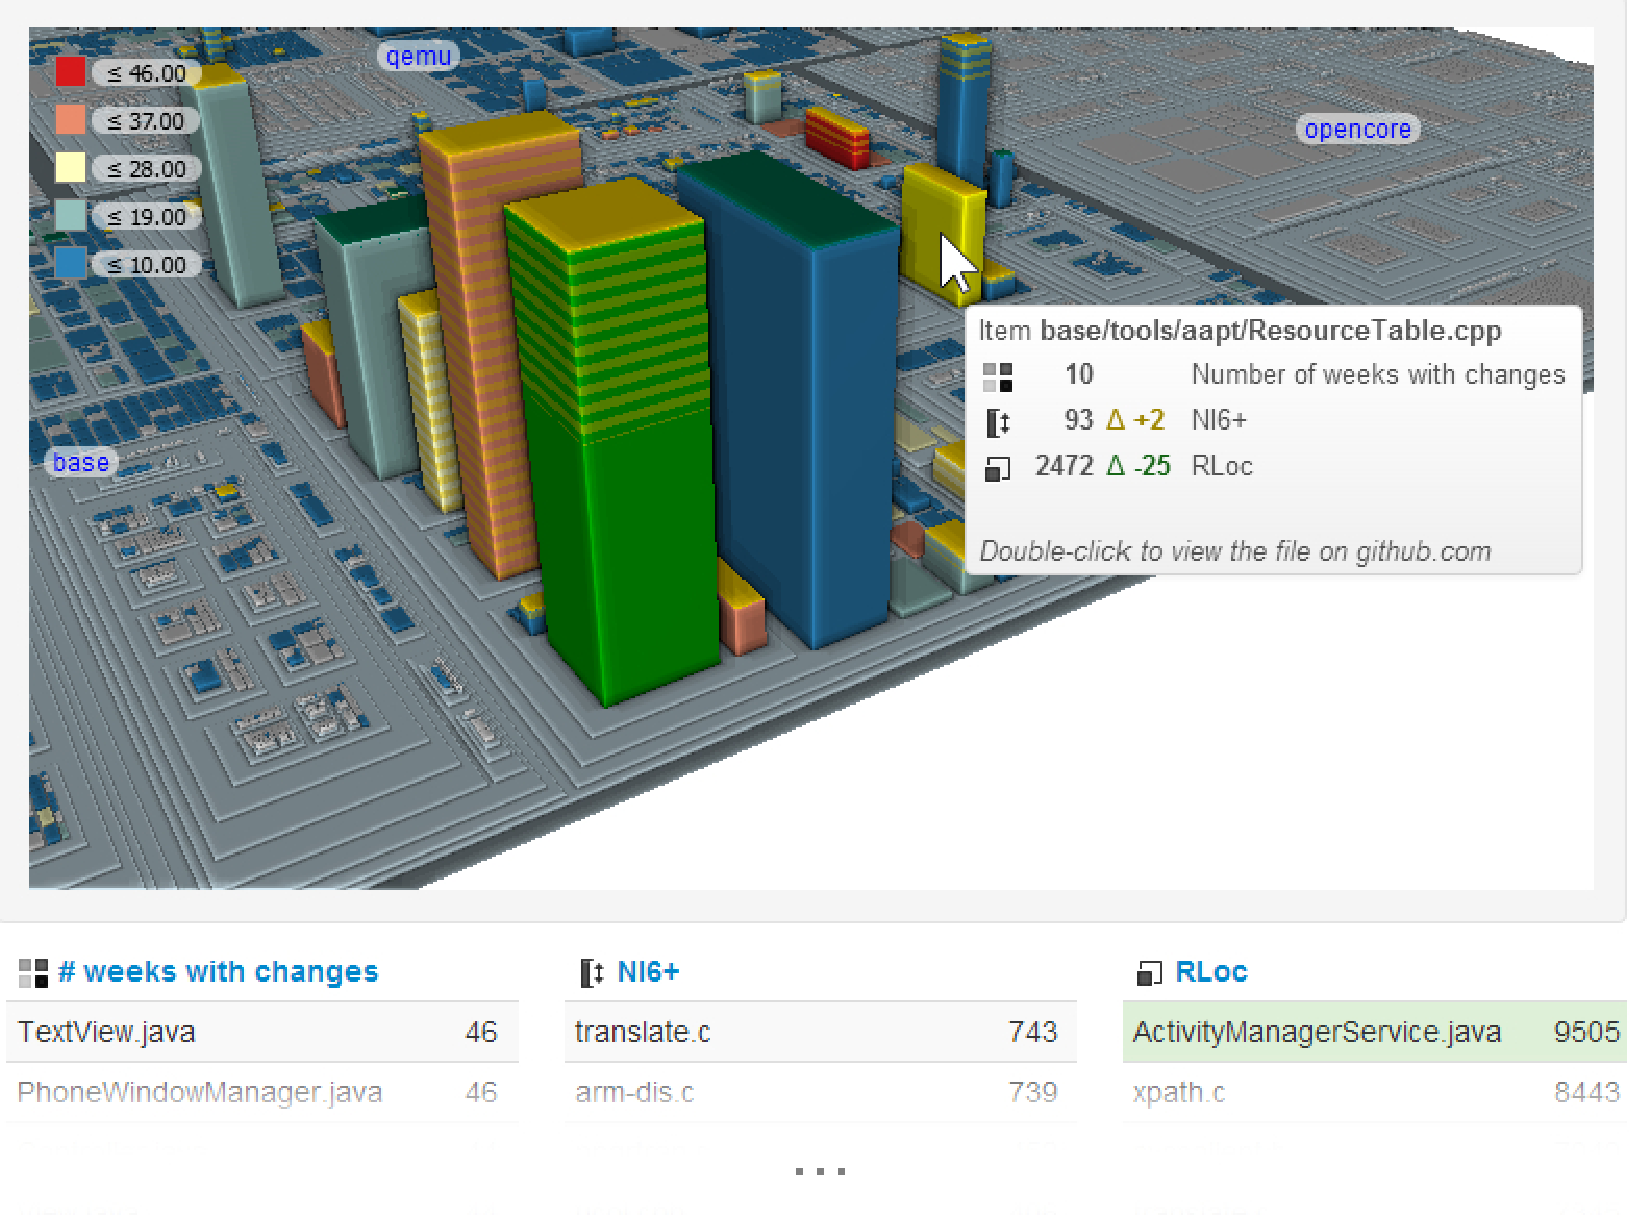
\includegraphics[width=1.0\linewidth]{figures/features3}
  \caption{This section shows various features of our visualization within the browser. In the upper part, importance-based, separate labeling of code units and modules is applied. In the center, a tooltip containing detailed information like exact metric values and differences, metric names, and the code unit's path or name. In addition, highlighting of user picked code units, visible as green code units in both item tables and visualization, is shown.
  In this case, the Android project is shown, for which attributes like, e.g., McCabe's complexity, real lines of code, coverage, or number of developers can be visualized.
    For example, the ActivityManagerService stands out with its high nesting level and RLoc count.
	It turns out that this item is regularly manipulated by many different developers and thus, could be considered as a potential quality risk.}
	\label{fig:features}	
\end{figure}

A software map, as a representation of a tree, consists of modules as nodes and items as leaves, both represented as boxes.
Modules represent directories or similar project structuring entities.
Items represent individual code units.
The height of an item is defined by the relative value of its assigned metric value whereas the height of a module is constant. 
The generic terms module and item are preferred to avoid confusion with project specific language and structure conventions.
Software projects based on ABAP\footnote{Advanced Business Application Programming language by SAP} for example, have no file structure but are based on tables and development objects or classes.
Most C++ projects, in contrast, are file-based projects with classes; commonly one principal class per header and source pair.

For the representation of the software map two data structures are used: a JSON-based \scite{Json2006} hierarchy and binary geometry data represented by typed arrays \scite{Khronos2012}.
Both are transmitted via AJAX requests in a compressed way (HTTP compression, i.e., GZIP \scite{Gzip1996}). 
This reduces the transmitted data by up to 65\% (Table \ref{tab:performance}).

\subsection{Hierarchy Data}

The hierarchy is a JSON structure, where the keys are item ids and the values are arrays with information about these items (Figure \ref{fig:jsonexample}).
The first entry is the \emph{box geometry index}: a pointer into the render geometry that is used for highlighting (i.e., to look up where in the color array the color for this specific item is stored so it can be exchanged for the highlight color) and interactive exploration.
The third entry is the item name.
To assemble the full item path (e.g., for the tooltip), the second entry, parent id, is used to recursively query the hierarchy and concatenate the item/module names.

Entries 4 to 9 are only present for items. 
They are the metric values and differences (between the last and current metric set) for the three mapping dimensions and are shown in tooltips (Figure \ref{fig:features}).

The complete hierarchy can become quite big, especially item/module names take up much space (Table \ref{tab:performance}).
To be able to show something quickly, we transmit the hierarchy in two parts. The first one is sent together with the so-called report.
The report contains meta information like project name, number of items, authors, revisions, the name of the perspective, metric names and explanations, and the ids of all labeled items and modules.
The hierarchy part of the report contains information about the $n$ (i.e., 20) top items per metric and all labeled items and modules.
The second part contains the whole hierarchy, the already transmitted items excluded.
Once report and geometry are loaded, \emph{top item tables} (Figure \ref{fig:webinterface}) and labels on the software map can be displayed.

\begin{figure}[b!]
  \centering
  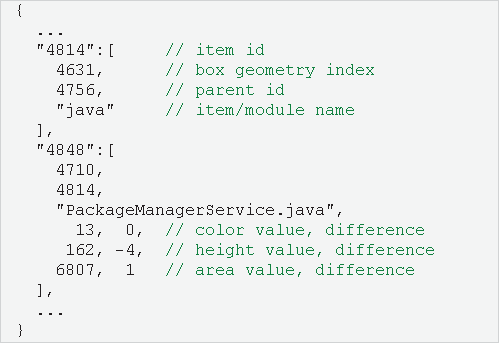
\includegraphics[width=1.0\linewidth]{figures/jsonexample}
  \caption{An exemplary excerpt of a JSON file, providing hierarchy and metrics information for the software map visualization.}
	\label{fig:jsonexample}
\end{figure}

\subsection{Geometry Data}

\begin{figure*}[ht]
  \centering
  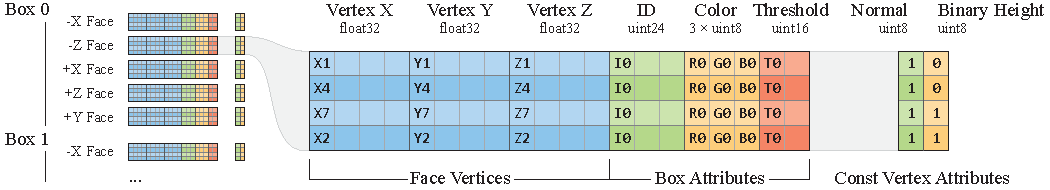
\includegraphics[width=1.0\linewidth]{figures/arrays}
  \caption{Drawing a software map chunk accesses a constant index array, two static arrays containing constant vertex attributes (normal as face attribute and binary height as vertex attribute), and chunk specific attribute arrays that contain vertex data and other box attributes. The illustration shows the memory size (one byte per block) and exemplary content of the arrays for the first box's second face of a chunk.}
	\label{fig:arrays}
\end{figure*}

The camera navigation is restricted to the upper hemisphere, making bottom faces unnecessary.
Even without the camera restriction, a single bottom face for the software map's root module would be sufficient.
Concerning attribution, the following attribute-geometry relations need to be taken into account: per-vertex, per-face, and per-box.
They need to be provided for the indexed vertices, yielding 30 indices per box and 20 vertices with attributes.
For rendering, we primarily need color, diff threshold, and id per box, normal per face, height per vertex, as well as a top vertex classification flag per vertex for diff rendering (\emph{binary height}).

In WebGL, vertex index buffers are currently limited to 16-bit indices.
Thus, a maximum of 65k vertices or $3\,276$ modules and items can be rendered per draw call.
Because software maps are usually significantly larger, they are rendered in chunks with a maximum of $65\,520$ vertices each.
Chunks do not need to have the same number of boxes, and a predefined ordering, providing more regular, continuous chunks as, e.g., rectangular shaped patches could be beneficial for frustum culling.
Contrarily, chunks are filled up in sequence as emerged by the hierarchy, keeping the number of required draw calls to a minimum and forgo time-consuming server or client-side reorganization of geometry data.

Since each chunk represents a sequence of boxes, the indexing remains the same for each chunk; 
Generating only one chunk and using it for all draw calls saves memory on the GPU.
During rendering, normals, binary heights, and indices are bound once, and the arrays for vertices, colors, and ids are re-bound for every draw call with a different offset (a multiple of the chunk size).
The various attribute relations demand a quad based triangle definition, resulting in a large redundancy for per-box and per-face attributes (Figure \ref{fig:arrays}).
Furthermore, indices need to be provided for drawing of single triangles, resulting in 6 indices per quad.

For the geometry, we transmit compact versions of the arrays used for rendering by a binary AJAX request (response type \emph{ArrayBuffer}).
Due to the regular structure of the axis-aligned boxes, indices, normals, and binary heights need not be transmitted, but can be generated on the client instead. 
There are four arrays remaining: vertices, colors, ids, diff thresholds.
They are stored consecutively and are each preceded by their length (int).
During loading, typed views into the received array buffer are created for processing the data.
Vertices are transferred as \emph{Float32Array}, containing bounding box information (llf and urb) only.
From this the full box geometry of 20 vertices (4 vertices per face, 5 faces) is created.
Colors and IDs are transferred as \emph{Uint8Arrays}, diff thresholds as \emph{Int16Array}.
They contain the values for each box in the same order as in the vertex array.
Since one box has 20 vertices, the data has to be replicated to new arrays, duplicating each date 20 times consecutively.
Figure \ref{fig:arrays} illustrates the content and memory footprint of all generated attribute arrays.

\section{Software-Map Rendering}

With image-based rendering and deferred stylization, imagery is generated by rendering attributed geometry into textures using render-to-texture while concurrently filling G-Buffers \scite{Saito1990}.
Rendering to multiple targets, however, is not available with WebGL yet (though an extension is in the works: WebGL\_draw\_buffers), limiting rendering of a single pass to a single G-Buffer.
Another limitation in WebGL is that the support for floating point textures is optional. 
Therefore float values (like depth) have to be encoded in four 8-bit channels (RGBA).
This section describes how G-Buffer data is encoded and used for stylization and exploration of large software maps. 

\subsection{Efficient Data Encoding}

\begin{figure*}[ht!]
  \centering
  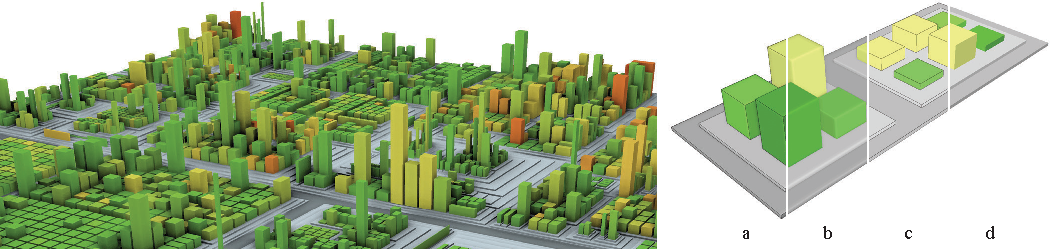
\includegraphics[width=1.0\linewidth]{figures/stylization}
  \caption{A composition of various stylization techniques supported by our rendering pipeline.
	The segments on the right show treemaps rendered with unsharp masking (b), edge enhancement (c), and static lighting (d).
	All three techniques are combined in the first segment (a).}
	\label{fig:stylization}
\end{figure*}

To enable the application of various image-based stylizations, a basic set of two common G-Buffers is provided.
The first contains colors and normals (\emph{rgbn-buffer}), the second linearized depths (\emph{depth-buffer}).
Box identities are rendered to a third G-Buffer (\emph{id-buffer}), that is mandatory for image-based interaction (i.e., hovering).

The rgbn-buffer contains color and normal information, all of which is encoded by four unsigned bytes.
The color calculation uses various vertex attributes and uniforms.
Color, diff threshold, binary height, highlight status, highlight and mouse-over colors, as well as a procedural texturing are exclusively processed in this pass.
Factors that are considered for color calculation are described in more detail in the following subsection.
Since only axis-aligned, five-sided boxes are rendered for the software map, only five distinct normals are required.
These are encoded by indices as follows: $\pm 2 \rightarrow \pm x$, $\pm 1 \rightarrow \pm z$, and $0 \rightarrow +y$.
The normal index is stored as an unsigned byte, which is provided as normalized float in $[0;1]$ within shaders.
Although no dynamic access to constant arrays within shaders is possible in WebGL, this scheme allows for efficient decoding without branching:
\\
\begin{lstlisting}
vec3 decodeNormal(in float i)
{
	i -= 2;
	float a = sign(i);
	return vec3(i - a, 1 - a * a, 2 * a - i);
}
\end{lstlisting}

The parameter i is expected in $\lbrack 0;4 \rbrack$ and encodes the normal of a single software-map face via signed indices $\{-2,-1, 0,+1,+2\}$. Its value specifies the vertex component and its sign the normal direction.

The id-buffer provides an unsigned 24-bit integer identity per box, encoded by three bytes.
It is used for fast object picking and further enables enhancement of various stylizations (i.e., edge enhancement).
The depth-buffer stores linearized depth values within the range $[0;1]$ and is encoded by three bytes as well.
Encoding of 32-bit floats to three single-byte channels, and vice versa, can be done within the shader as follows:
\\
\begin{lstlisting}
vec3 float2vec3i(const in float f)
{
  return vec3(
    floor(      f *   256.0)          / 255.0,
    floor(fract(f *   256.0) * 256.0) / 255.0,
    floor(fract(f * 65536.0) * 256.0) / 255.0);
}
float vec3i2float(const in vec4 v)
{
  return v[0] * 255.0 / (256.0)
       + v[1] * 255.0 / (256.0 * 256.0)
       + v[2] * 255.0 / (256.0 * 256.0 * 256.0);
}
\end{lstlisting}

To enhance human perception of the software-map hierarchy and to facilitate visual distinction of individual code units, a composition of various stylization techniques can be applied (Figure \ref{fig:stylization}):
Static lighting, edge enhancements through contour lines \scite{Nienhaus2003}, and either unsharp masking \scite{Luft2006} or any efficient screen space ambient occlusion (SSAO).

Static lighting often uses a distant light at the camera's position \scite{Trapp2013}. 
For software maps, we suggest fixating the camera at a constant altitude.
This yields a constant, view independent coloring of the software-map's top faces (i.e., all horizontal faces), and further reduces the overall light variation for vertical faces due to camera movement.
Colors remain stable for top faces and can be adjusted to exactly match the color scheme (visual matching of colors of vertical faces becomes also more accurate).

For edge enhancement, contours generated from normal, color, and id buffers are used to add colored contour lines to all visible edges of each box.
Depth-buffer unsharp masking increases depth cues and the overall visual quality.
Alternatively, SSAO can be used, which further increases the perceived plasticity of the software map.
In Figure \ref{fig:features}, unsharp masking was used, compared with a more expensive SSAO used in Figure \ref{fig:stylization}.
Illumination that affects saturation or hue (e.g., color bleeding as result of global illumination) is not recommended, since it obviously distorts the perceptual color mapping and thereby hinder accurately reading metrics encoded in color.

It is often difficult to discern the basic structure of the code base (i.e., the root modules) even with basic padding applied to the treemap layout.
To alleviate this, we increase the border between root modules and color it differently (i.e., darker, with neither saturation nor hue change -- Figure \ref{fig:stylization}).
Since the interesting modules may not be at the top hierarchy level, we can adjust the hierarchy level that is considered the root level.

\subsection{Interactive Exploration}

A meaningful exploration of software maps requires interactions and displaying of information to be aligned to one another and highly adjusted to the targeted use cases.
This section discusses technical details of labeling, highlighting and hovering, tooltips provisioning, and difference visualization, that is the visual emphasis of metric changes.

Small textual annotations of software map artifacts are commonly referred to as \emph{labels}.
The process of controlled label placement is \emph{labeling}.
We provide multiple ways to find or identify a code unit within the software map: 
Labeling of top items, labeling of root (or similarly discernible) modules, highlighting via batch selection in \emph{top item lists}, and provision of tooltips for individual items (Figure \ref{fig:features}, with black/blue labels in the figure referring to item and module labels).
The labeling of software maps is similar to the labeling of geovirtual 3D-environments, since both feature a two dimensional spatial context enriched with height information. 

Item labels are connected to their boxes via poles; if they overlap, labels farther away from the camera are moved upwards.
We therefore rely on a technique that places labels such that they avoid occluding one another\scite{Hagedorn2007}.
Module labels work slightly different as they are not connected via a pole.
Instead, the mental connection to the labeled module is achieved by placing it in the center of the module.
Also, we hide module labels if they would be moved more than half of its height since the mental identification with the labeled module can easily get lost if it is not centered properly.
To ensure that labels of large modules are not hidden by labels of smaller modules, we sort the labels by module area in descending order before rendering.
While the number of shown item labels is a system setting, the number of shown module labels is view-dependent, i.e., labels for smaller modules can be made visible by zooming in.

The camera navigation for software maps is based on and thus similar to common terrain navigation (e.g., Google Earth).
It supports panning, zooming, and rotation, wherein the first two require depth buffer access for fulfilling individual constraints.

When a user starts panning, the initial intersection point is used as a reference point and required to remain exactly below the mouse cursor.
This is contrary to intersecting with the ground plane, since panning can be initiated by picking a side face at arbitrary height, necessitating a correct panning speed.
The first click of the interaction is used to access the depth-buffer and to retrieve the related object-space position $p_0$.
This point is our constraint for panning, which means that for every mouse position there has to be an appropriate positioning for the software map, so that the point under the cursor remains $p_0$.
With this point and the up normal we build a plane, that defines the panning space.
For panning, a ray is created, pointing from the screen pixel into the view frustum.
This ray then is converted to object space and used to intersect with the plane at $p$.
The delta of $p_0$ and $p$ is the translation required for our constrained panning.
We further require at least one single fragment of the software map to be at the viewport's center by constraining the software-map's center to its own bounding box.

Rotation is applied around the software map's central y-axis, since we found users to be disturbed when rotation is around y-aligned axes centered at the initial intersection points.
Furthermore, vertical rotation is restricted by a minimum angle to a range above the horizon, and a minimum angular distance to the up vector.
This prevents seeing the software map from below or upside down.

For zooming, the camera should move with respect to the pointed software-map position.
This is done by scaling the distance between the pointed position in the scene (again via depth-buffer) and the camera position.
Since the software-map's center needs to be constrained to the ground plane, a temporary center is calculated based on the initial intersection with the ground plane and then used to obtain the new viewray-groundplane intersection as new center.
With that, zooming can be deliberately used to pan and scale towards a module's or item's top or side face.
This approach allows fast transitions to arbitrary places of interest by zooming only, thus increasing navigation efficiency.
For mobile use, i.e., devices with touch enabled displays, a simple mapping of common touch gestures is used (pinch is simultaneously used for rotation and zoom).

Two other aspects of software map exploration are hovering and highlighting.
The first causes a recoloring of the hovered item or module for the time being hovered.
The second can be applied for multiple items, by batch-selecting items in the \emph{top item lists}.
The item's basic color is retrieved from the color attribute and replaced by the hover color, if the item is hovered. 
Additionally, if the compare threshold attribute contains a valid value, a procedural texture (i.e., horizontal stripes) is applied to mark the difference between the current and the old metric value (yellow stripes as in Figure \ref{fig:features}).
Finally, double clicking items browses the linked source code and tooltips are used to provide more detailed information for an item.

\section{Discussion and Results}

\begin{table}[b!]
	\begin{tabular*}{\linewidth}{@{\extracolsep{\fill}}lrr}
		\toprule
			& Android & Customer Project \\
		\midrule

		Code Units \#     &  30\,853  &     90\,089 \\
		\addlinespace

		Vertices \#       & 617\,060  & 1\,801\,780 \\
		Triangles \#      & 308\,530  &    900\,890 \\
		\addlinespace

		geometry.bin      &  964 KiB  &  2\,815 KiB \\
		\small
		compressed$^*$ & \small 404 KiB / 19 ms / 3 ms & \small 1\,175 KiB / 56 ms / 11 ms	\\
		\small 
		compression ratio & \small 0.42 & \small 0.42 \\	
		\addlinespace

		report.json       &    4 KiB  & 16 KiB \\
		\small 
		compressed$^*$ & \small 2 KiB / 0 ms / 0 ms	& \small 7 KiB / 0 ms / 0 ms \\
		\small
		compression ratio & \small 0.51	& \small 0.45 \\
		\addlinespace

		hierarchy.json    & 1\,513 KiB  &  5\,429 KiB\\
		\small
		compressed$^*$	& \small 480 KiB / 21 ms / 6 ms	& \small 1\,587 KiB / 70 ms / 19 ms \\
		\small
		compression ratio & \small 0.32 & \small 0.29 \\
		\addlinespace

		GPU Memory        & 12.082 MiB  & 34.679 MiB \\
		\bottomrule

		\multicolumn{3}{l}{\small $^*$gzip (zlib) compression level 1, with compress and decompress times.}\\
	\end{tabular*}
	\caption{
		Listed are file sizes of all files required for the visualization.
		System: Intel Xeon CPU E5-1620 0 at 3.6\,GHz. }
	\label{tab:performance}
\end{table}

The presented visualization is applicable to similar techniques like CodeCities\scite{Wettel2007a} and scales up to real-world software projects containing up to 90k code units (Table \ref{tab:performance}).
Although large code bases might contain more code units, applying a one-to-one mapping from code units to treemap items is not useful then: Visual clutter (e.g., too small individual items, occlusion) begins to increase drastically, which generally renders software maps unusable.
Hence, pre-filtering of input data -- to reduce the number of code units to approx. 100k -- has to take place anyway, so that the scalability of our system is sufficient even for larger code bases.

The precision of the depth buffer varies throughout different hardware platforms, on some systems resulting in tiny discontinuities, causing visual artifacts on depth-buffer-based post processing (unsharp masking, SSAO).

To ensure the highest possible compatibility while providing good performance on powerful machines like desktop computers with dedicated graphics cards, it will become necessary to provide a baseline functionality based on WebGL 1.0 with optional optimized code paths that make use of the available extensions if they are available.
For example, with WebGL\_depth\_texture we could skip the depth pass and use the depth buffer from the color pass for SSAO.
Reducing the number of geometry passes from two to one is very useful, since for large projects ($>$ 50k items) the rendering speed is geometry-bound.
With OES\_element\_index\_uint we could increase the chunk size to a few million vertices.
The chunked rendering code would remain active (for systems without this extension), but effectively only one chunk would be rendered.

\begin{table}[t!]
	\begin{tabular*}{\linewidth}{@{\extracolsep{\fill}}lrr}
		\toprule
			& Android & Customer Project \\
		\midrule
		\addlinespace

		\small Transmission at 1.5 Mbps (synthetic):  & & \\
		Geometry + Report  & 5.04 s & 14.75 s \\
		Hierarchy          & 7.88 s & 28.28 s \\

		\small Transmission at 7.6 Mbps (synthetic):  & & \\
		Geometry + Report  & 1.00 s &  2.91 s \\
		Hierarchy          & 1.55 s &  5.58 s \\

		\small Local initialization on i5-3337U: & & \\
		Interface          &  0.24 s  & 0.24 s \\
		Geometry + Report  &  0.48 s  & 2.13 s \\
		Hierarchy          &  1.11 s  & 4.27 s \\
		\addlinespace

		\small Averaged frame rendering time: & & \\
		Intel HD Graphics 4000      & 5.62 ms  &  28.06 ms \\
		\small Intel Core i5-3337U at 1.80 GHz (WIN) & & \\
		NVIDIA GeForce GT 650M      & 1.92 ms  &  13.62 ms \\
		\small Intel Core i7 at 2.80 GHz (OS X) & & \\
		NVidia GTX 680              & 2.20 ms  &  16.04 ms \\
		\small Intel Xeon W3530 at 2.80 GHz (WIN)   & & \\
	\bottomrule
	\end{tabular*}
	\caption{	
		Listed are transmission, initialization, and average times per frame for rendering software maps of the two previous projects.
		Transmission and initialization times were measured separately, since the software map is available for interaction with geometry and report data provided, except for tool tips.
		Local initialization times were measured with Google Chrome's tracing capability, the influence of the tracing itself is ignored.
		The frame times were averaged across 1000 frames of continuous redraw with no interaction (by default, redraw is only triggered on interaction).
		Chrome 26.0.1410.64 was used as browser (WebKit 537.31, JavaScript V8 3.16.14.11).
		The resolution of the website was $1024 \times 1280$ and of the OpenGL canvas $976 \times 732$ pixels. 
		For Windows, ANGLE was utilized by Chrome, which surprisingly performed faster than direct OpenGL rendering.
		}
	\label{tab:frametimes}
\end{table}

Concerning rendering performance, we measured transmission, initialization and frame rendering times on three platforms: one ultrabook, one MacBook Pro, and one workstation.
For all devices, interactive frame rates have been met and transmission and initialization delays are reasonably fast within our use cases (Table \ref{tab:frametimes}).

\section{Conclusion and Future Work}

We have presented a web-based system for the interactive display and analysis of large software maps.
We achieve this technical scalability by efficiently encoding the data transferred to the client and by optimized usage of vertex attribute arrays.
We further address visual scalability of the software-map rendering by applying an importance-based LOD-filtering for labels that annotate treemap items.
A combination of interaction techniques for easy manipulation of the camera as well as details-on-demand features for querying additional properties of individual treemap items are provided.

Introducing filtering for modules, metrics, developers, code units etc. on the client side would be beneficial for the visualization's exploratory nature.
Layouting and configurable attribute mapping allowing for arbitrary metric-mapping parametrization from within the browser could increase the scope of web-based software-map analysis further.
Concerning data provisioning, we found that general-purpose storage containers (e.g., \scite{Behr2010}, \scite{Behr2012}, \scite{Jung2013}) can be useful in most rendering scenarios; however, they do not provide the efficiency of our approach (two vertices per box, various attributes, decoupled hierarchy, etc.).

The availability of a web-based software-map implementation now allows for connecting software maps to collaboration platforms, such as Github\footnote{\url{http://www.github.com}}, which improves user experience and lowers the access barrier.
With the centralized provisioning of (predefined) perspectives, users can now collaboratively re-use perspectives without being forced to define any themselves.
We hope more APIs promoting interactive web-based software maps or similar visualizations become available, making software visualization more accessible and supporting today's software engineering processes.

\section*{Acknowledgements}

We thank Software Diagnostics GmbH\footnote{\url{http://www.softwarediagnostics.com}}, for sharing their ideas and providing us access to their Software Diagnostics Transparency Platform.
This work was partially funded by the Federal Ministry of Education and Research (BMBF), Germany within the InnoProfile Transfer research group ``4DnD-Vis''.

\bibliographystyle{acmsiggraph}
\bibliography{web3d-webbased-treemaps}
\end{document}